\documentclass[a4paper]{article}     
\usepackage{amsfonts}
\usepackage{amsmath}
\usepackage{amssymb}
\usepackage{graphicx}
\usepackage{cancel}

\newcommand{\asa}{\Leftrightarrow} %als slechts als
\newcommand{\adR}{\Rightarrow} %als dan Rechts
\newcommand{\adL}{\Leftarrow}
\newcommand{\Lh}{\left(} %Links haakje
\newcommand{\Rh}{\right)}
\newcommand{\Lv}{\left[} %Links vierkanthaakje
\newcommand{\Rv}{\right]}
\newcommand{\La}{\left\{} %Links acolade
\newcommand{\Ra}{\right\}}
\newcommand{\Ras}{\right.} %Rechts acolade stelsel (omdat om stelsels te maken heb je een punt nodig
\newcommand{\pnR}{\rightarrow} %pijl naar Rechts
\newcommand{\limiet}{\lim\limits_}
\newcommand{\schrap}{\cancel}
\newcommand{\schrapb}{\bcancel} %backslash
\newcommand{\schrapk}{\xcancel} %kruis
\newcommand{\vervang}{\cancelto}
\newcommand{\intgrl}{\displaystyle\int} %integraal teken (bij het berekenen van primitieven)

\begin{document}

\noindent \large Auteur: Yoren Collier \\
\noindent \large Studierichting: Informatica\\
\noindent \large Oefeningenreeks 5D nr. 4.5\\

\medskip

\normalsize

Bereken het gebied tussen de krommen.\\

$y = x^2$ en $y = 3x$\\

$x^2 = 3x \asa x^2 -3x = 0 \asa x(x-3) = 0 \adR x=0$ of $x=3$\\

Stel: $x=1$\\  

$\left.
\begin{array}{l}
y = 1^2 = 1\\
y = 3 \cdot 1 = 3
\end{array}
\Ra
\adR$
in het gebied ligt $y = 3x$ hoger.\\

$ BI \intgrl_{0}^3 \Lh 3x -x^2 \Rh dx \adR OBI = \intgrl \Lh  3x -x^2 \Rh dx$\\

$= \dfrac{3 x^2}{2} - \dfrac{x^3}{3} +c$\\

$BI = \Lv \dfrac{3 x^2}{2} - \dfrac{x^3}{3}\Rv_{0}^3 = \dfrac{3}{2} \cdot 9 - \dfrac{1}{\schrap{3}} \cdot \vervang{9}{27} = \dfrac{27}{2} - 9 = \dfrac{27 - 18}{2} = \dfrac{9}{2} $\\

\begin{figure}[h]
\centering
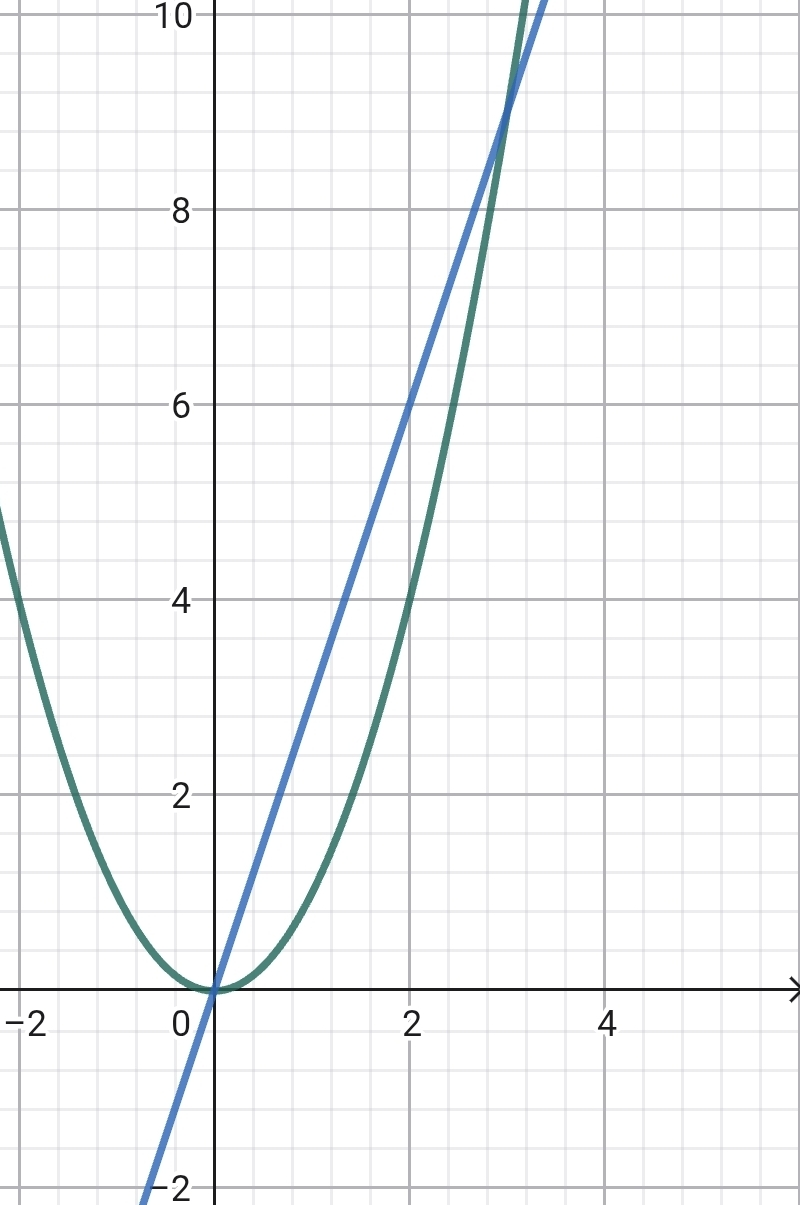
\includegraphics[width=10cm]{./5D-4.5-yoren.collier.INF.jpg}
\end{figure}

\begin{thebibliography}{999}
%\bibitem{a} Referentie
\end{thebibliography}
\end{document} 